\chapter{Signaling Pathway Activities Improve Prognosis for Breast Cancer}
\label{chap:hipathia}

\begin{chapabstract}

\textrm{{\bf Abstract:}} With the advent of high-throughput technologies for genome-wide expression profiling, a large number of methods have been proposed to discover gene-based signatures as biomarkers to guide cancer prognosis. However, it is often difficult to interpret the list of genes in a prognostic signature regarding the underlying biological processes responsible for disease progression or therapeutic response. A particularly interesting alternative to gene-based biomarkers is mechanistic biomarkers, derived from signaling pathway activities, which are known to play a key role in cancer progression and thus provide more informative insights into cellular functions involved in cancer mechanism. In this chapter, we demonstrate that a pathway-level feature, such as the activity of signaling circuits, outperform conventional gene-level features in prediction performance in breast cancer prognosis. We also show that the proposed classification scheme can even suggest, in addition to relevant signaling circuits related to disease outcome, a list of genes that do not code for signaling proteins whose contribution to cancer prognosis potentially supplements the mechanisms detected by pathway analysis. This study is under submission as joint work with Marta R. Hidalgo, Cankut \c{C}ubuk, Alicia Amadoz, Jos\'{e} Carbonell-Caballero, Jean-Philippe Vert, Joaqu\'{i}n Dopazo \cite{Jiao2017Signaling}.
\linebreak
\vskip 0.1in
\noindent \textrm{{\bf R�sum� :}}

\end{chapabstract}

\section{Introduction}
\label{sec4:intro}

Over the past decades, many efforts have been addressed to the identification of gene-based signatures to predict  patient prognosis using gene expression data \cite{Veer2002Gene, Paik2004multigene, Wang2005Gene, Sotiriou2009Gene, Reis-Filho2011Gene}. Despite the success of its use, gene expression signatures have not been exempt of problems \cite{Ein-Dor2006Thousands, Iwamoto2010Predicting}. Specifically, one major drawback of multi-gene biomarkers is that they often lack proper interpretation in terms of mechanistic link to the fundamental cell processes responsible for disease progression or therapeutic response \cite{Veer2008Enabling, Dopazo2010Functional}. Actually, it is increasingly recognized that complex traits, such as disease or drug response, are better understood as alterations in the operation of functional modules caused by different combinations of gene perturbations \cite{Barabasi2004Network, Oti2007modular, Barabasi2011Network}. To address this inherent complexity different methodologies have tried to exploit several functional module conceptual representations, such as protein interaction networks or pathways, to interpret gene expression data within a systems biology context \cite{Barabasi2011Network, Vidal2011Interactome, Hood2013Systems, Fryburg2014Systems}.

Here we focus on consulting prior knowledge of signaling pathways to guide cancer prognosis. It is well understood that cell signaling is a system of within-cell communication and signal transduction process between gene products, mostly proteins, that coordinates cell activities to perceive and correctly respond to microenvironment, resulting in signaling pathways that form a particular type of functional gene modules and play a key role in disease progression (Figure \ref{fig4:cellsignaling}). Consequently as a tempting solution to the limitation of conventional analysis at the level of individual genes, analysis at the level of pathways renders great interest in providing informative insights into cellular functions that facilitates understanding of the disease mechanism. Actually, it has recently been shown that the pathway-level representation generates clinically relevant stratifications and outcome predictors for glioblastoma and colorectal cancer \cite{Drier2013Pathway} and also breast cancer \cite{Livshits2015Pathway}. Moreover, mathematical models of the activity of a pathway have demonstrated a significantly better association to poor prognosis in neuroblastoma patients than the activity of their constituent genes, including MICN, a conventional biomarker \cite{Fey2015Signaling}. This observation has recently been extended to other cancers \cite{Hidalgo2017High} and to the prediction of drug effects \cite{Amadoz2015Using}.

\begin{figure}[!htbp]
	\centering
	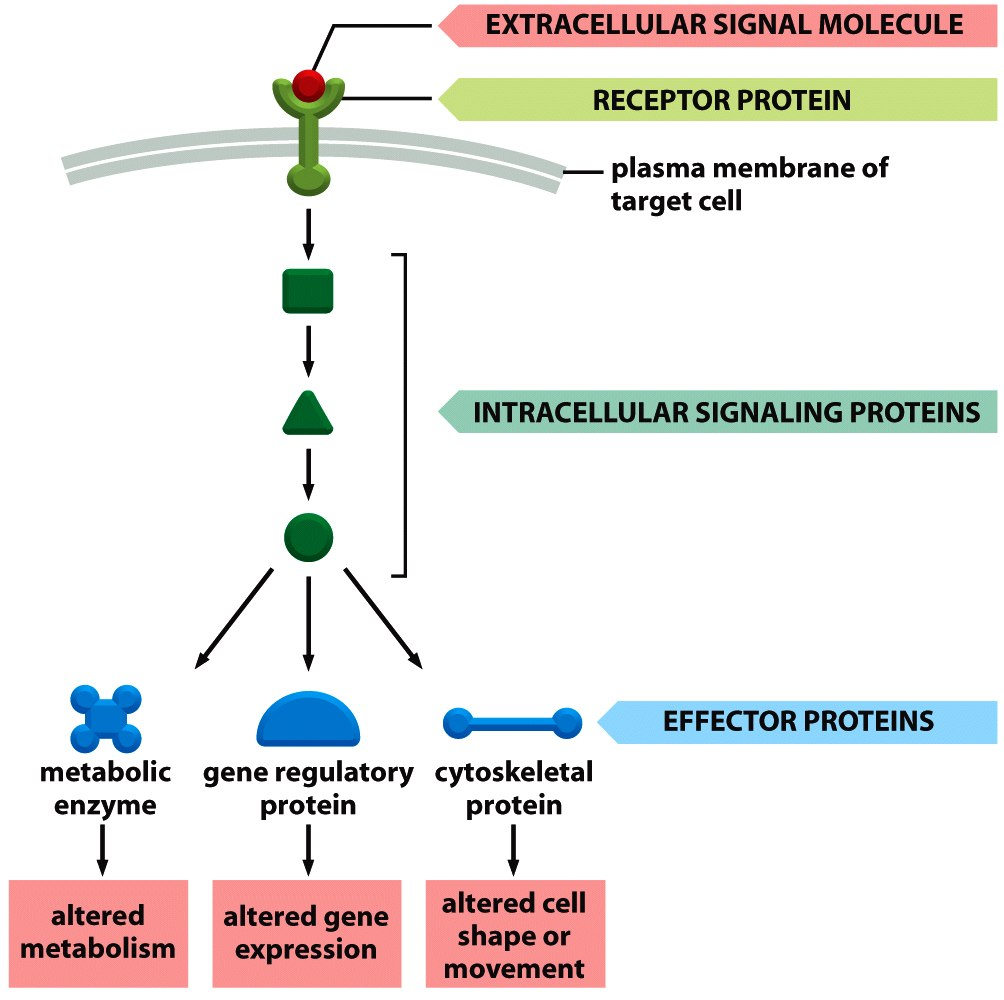
\includegraphics[width=0.6\textwidth]{ch-hipathia/figure/signaling_pathway}
	\caption{An illustration of cell signaling process. Typically the signal transduction begins at receptor proteins that receive molecular stimuli from cell microenvironment and ends at effector proteins that execute specific actions in response to the stimulation.}
	\label{fig4:cellsignaling}
\end{figure}

Given that the inferred activity of the pathway should be closely related to its cellular mechanism for disease progression, its use to guide cancer prognosis seems promising. Recently, a number of pathway activity inference methods have been proposed \cite{Hidalgo2017High, Jacob2012More, Li2015Subpathway, Martini2013Along}. Here, we use the \textit{hiPathia} method proposed in \cite{Hidalgo2017High}, as it has been demonstrated to have a superior performance finding significant associations of specific circuit\footnote{Circuits can be understood as sub-pathways with specific  structure in stimulus-response signaling pathways, while definitions are postponed to Section \ref{sec4:hipathia}.} activities, directly responsible for triggering the prominent cancer hallmarks \cite{Hanahan2011Hallmarks}, to patient survival. This method recodes gene expression values into measurements of signaling circuit activities that ultimately account for cell responses to specific stimuli. Such activity values can be considered multigenic mechanistic biomarkers that can be used as features for cancer prognosis.

In this chapter, we demonstrate that the activity of signaling circuits yields comparable or even better prediction in breast cancer prognosis than the expression of individual genes, while detected mechanistic biomarkers enjoy the compelling advantage of readily available interpretation in terms of the corresponding cellular functions they trigger. Moreover, we show that the proposed prediction scheme can even suggest, in addition to interesting signaling circuits related to disease outcome, a list of genes that do not code for signaling proteins whose contribution to cancer prognosis potentially supplements the mechanism included in the pathways modeled. All numerical results are produced with \texttt{R} and codes for reproducing the experiments are available in the online supplementaries at \url{https://github.com/YunlongJiao/hipathiaCancerPrognosis}.




\section{Methods}
\label{sec4:methods}

\subsection{Data Source and Processing}
\label{sec4:data}

Our interest in this study lies in predicting the overall survival outcome of breast cancer patients making use of gene expression data. The breast cancer gene expression and survival data here were downloaded from The Cancer Genome Atlas (TCGA), release No. 20 of the International Cancer Genome Consortium (ICGC) data portal under project name BRCA-US\footnote{More information can be found at \url{https://dcc.icgc.org/releases/release_20/Projects/BRCA-US}.}. This dataset provides the RNA-seq counts of 18,708 genes for 879 tumor samples in which we also have records of the vital status of corresponding donors, namely the overall survival outcome of the cancer patients being alive or deceased at the end of clinical treatment (Table \ref{tab4:survival}). This way we deal with a binary classification problem distinguishing good vs poor prognosis based on gene expression measurements of breast tumor samples. Since TCGA cancer data are collected from different origins and underwent different management processes, non-biological experimental variations, commonly known as batch effect, associated to Genome Characterization Center (GCC) and plate ID must be removed from the RNA-seq data. The COMBAT method \cite{Johnson2007Adjusting} was used for this purpose. We then applied the trimmed mean of M-values normalization method (TMM) method \cite{Robinson2010scaling} for data normalization which is essential in applying the \textit{hiPathia} method. The resulting normalized values were finally entered to the pathway analysis method.

\begin{table}[!htbp]
	\centering
	\caption{Summary of survival outcome of the breast cancer patients in the TCGA dataset.}
	\begin{tabular}{|l|l|r|r|}
		\hline
		\textbf{Donor vital status} & \textbf{Pseudo label} & \textbf{No. of samples} & \textbf{Percentage} \\
		\hline
		Deceased (poor prognosis) & Positive & 124 & 14.1\% \\\hline
		Alive (good prognosis) & Negative & 755 & 85.9\% \\\hline
		\multicolumn{2}{|r|}{\textbf{Total}} & 879 & 100.0\% \\
		\hline
	\end{tabular}
	\label{tab4:survival}
\end{table}

In order to explore the potential of utilizing external knowledge of cell signaling to enhance prognosis, we consulted Kyoto Encyclopedia of Genes and Genomes (KEGG) repository \cite{Kanehisa2012KEGG} to retrieve relationships between proteins within signaling pathways. A total of 60 KEGG pathways were used (Table \ref{tab4:kegg}), comprehending 2,212 gene products that participate in 3,379 nodes. Note that most gene products are proteins, and two types of nodes are defined in KEGG: plain nodes which may contain one or more proteins and complex nodes. These pathways each compose into a directed network where nodes are connected with edges labeled by either activation or inhibition depending on the action in transmitting signals along the path. In particular, input nodes that have no incoming edges represent receptor proteins which receive molecular stimuli from cell microenvironment, and output nodes that have no outgoing edges represent effector proteins which carry out specific cellular functions. We will elaborate in the following subsection on how to decompose the complex structure of KEGG pathways in order to effectively apply the \textit{hiPathia} method.

\begin{center}
	\begin{longtable}[H]{|l|l|}
	\caption{The 60 KEGG pathways for which signaling activity is modeled.}
	\label{tab4:kegg}\\
		
		\hline \multicolumn{1}{|l|}{\textbf{KEGG identifier}} & \multicolumn{1}{l|}{\textbf{Pathway name}} \\ \hline 
		\endfirsthead
		
		\multicolumn{2}{c}%
		{{\tablename\ \thetable{} -- continued from previous page}} \\
		\hline \multicolumn{1}{|l|}{\textbf{KEGG identifier}} & \multicolumn{1}{l|}{\textbf{Pathway name}} \\ \hline 
		\endhead
		
		\multicolumn{2}{|r|}{\textit{Continued on next page}} \\ \hline
		\endfoot
		
		\hline
		\endlastfoot
		
		hsa04014 &
		Ras signaling pathway \\\hline
		hsa04015 &
		Rap1 signaling pathway \\\hline
		hsa04010 &
		MAPK signaling pathway \\\hline
		hsa04012 &
		ErbB signaling pathway \\\hline
		hsa04310 &
		Wnt signaling pathway \\\hline
		hsa04330 &
		Notch signaling pathway \\\hline
		hsa04340 &
		Hedgehog signaling pathway \\\hline
		hsa04350 &
		TGF-beta signaling pathway \\\hline
		hsa04390 &
		Hippo signaling pathway \\\hline
		hsa04370 &
		VEGF signaling pathway \\\hline
		hsa04630 &
		Jak-STAT signaling pathway \\\hline
		hsa04064 &
		NF-kappa B signaling pathway \\\hline
		hsa04668 &
		TNF signaling pathway \\\hline
		hsa04066 &
		HIF-1 signaling pathway \\\hline
		hsa04068 &
		FoxO signaling pathway \\\hline
		hsa04020 &
		Calcium signaling pathway \\\hline
		hsa04071 &
		Sphingolipid signaling pathway \\\hline
		hsa04024 &
		cAMP signaling pathway \\\hline
		hsa04022 &
		cGMP-PKG signaling pathway \\\hline
		hsa04151 &
		PI3K-Akt signaling pathway \\\hline
		hsa04152 &
		AMPK signaling pathway \\\hline
		hsa04150 &
		mTOR signaling pathway \\\hline
		hsa04110 &
		Cell cycle \\\hline
		hsa04114 &
		Oocyte meiosis \\\hline
		hsa04210 &
		Apoptosis \\\hline
		hsa04115 &
		p53 signaling pathway \\\hline
		hsa04510 &
		Focal adhesion \\\hline
		hsa04520 &
		Adherens junction \\\hline
		hsa04530 &
		Tight junction \\\hline
		hsa04540 &
		Gap junction \\\hline
		hsa04611 &
		Platelet activation \\\hline
		hsa04620 &
		Toll-like receptor signaling pathway \\\hline
		hsa04621 &
		NOD-like receptor signaling pathway \\\hline
		hsa04622 &
		RIG-I-like receptor signaling pathway \\\hline
		hsa04650 &
		Natural killer cell mediated cytotoxicity \\\hline
		hsa04660 &
		T cell receptor signaling pathway \\\hline
		hsa04662 &
		B cell receptor signaling pathway \\\hline
		hsa04664 &
		Fc epsilon RI signaling pathway \\\hline
		hsa04666 &
		Fc gamma R-mediated phagocytosis \\\hline
		hsa04670 &
		Leukocyte transendothelial migration \\\hline
		hsa04062 &
		Chemokine signaling pathway \\\hline
		hsa04910 &
		Insulin signaling pathway \\\hline
		hsa04922 &
		Glucagon signaling pathway \\\hline
		hsa04920 &
		Adipocytokine signaling pathway \\\hline
		hsa03320 &
		PPAR signaling pathway \\\hline
		hsa04912 &
		GnRH signaling pathway \\\hline
		hsa04915 &
		Estrogen signaling pathway \\\hline
		hsa04914 &
		Progesterone-mediated oocyte maturation \\\hline
		hsa04921 &
		Oxytocin signaling pathway \\\hline
		hsa04919 &
		Thyroid hormone signaling pathway \\\hline
		hsa04916 &
		Melanogenesis \\\hline
		hsa04261 &
		Adrenergic signaling in cardiomyocytes \\\hline
		hsa04270 &
		Vascular smooth muscle contraction \\\hline
		hsa04722 &
		Neurotrophin signaling pathway \\\hline
		hsa05200 &
		Pathways in cancer \\\hline
		hsa05231 &
		Choline metabolism in cancer \\\hline
		hsa05202 &
		Transcriptional misregulation in cancer \\\hline
		hsa05205 &
		Proteoglycans in cancer \\\hline
		hsa04971 &
		Gastric acid secretion \\\hline
		hsa05160 &
		Hepatitis C
	\end{longtable}
\end{center}

\subsection{Modeling Framework for Signaling Pathways}
\label{sec4:hipathia}

We applied the \textit{hiPathia} method\footnote{Available as an \texttt{R} package at \url{https://github.com/babelomics/hipathia} and via a web interface at \url{http://hipathia.babelomics.org/}.} proposed by \cite{Hidalgo2017High} in pursuit of modeling signaling activity. Overall, \textit{hiPathia} is a method that estimates the level of activity within a signaling circuit by modeling cell signaling process in order to recode gene expression values into measurements that ultimately account for cell responses caused by pathway activities. Essentially the \textit{hiPathia} method computes an activity value for each stimulus-response sub-pathway within signaling circuits. This way, the sub-pathways which associate naturally with cell functionalities can be considered as mechanistic features that are modularized from multigenic signatures, and their activity values connected to the activation or deactivation of specific cellular functions thus provide quantitative clues to understand disease mechanisms when further related to phenotypes of interest such as cancer survival.

Recall that in cell signaling process represented in KEGG pathways, cell signal arrives to an initial input node and starts to transmit along any path following the direction of the edges until it reaches an output node that finally triggers a cellular action. In particular, from different input nodes the signal may follow different routes to reach different output nodes. Within the modeling context, a \textit{circuit} is naturally defined as all possible routes the signal can traverse to be transmitted from a particular input node to a particular output node (Figure \ref{fig4:pathway}, A). A total of 6,101 circuits are identified and modeled in this study. Now we take efforts to describe first how \textit{hiPathia} estimates the signaling activity of a circuit.

\begin{figure}[!htbp]
\centering
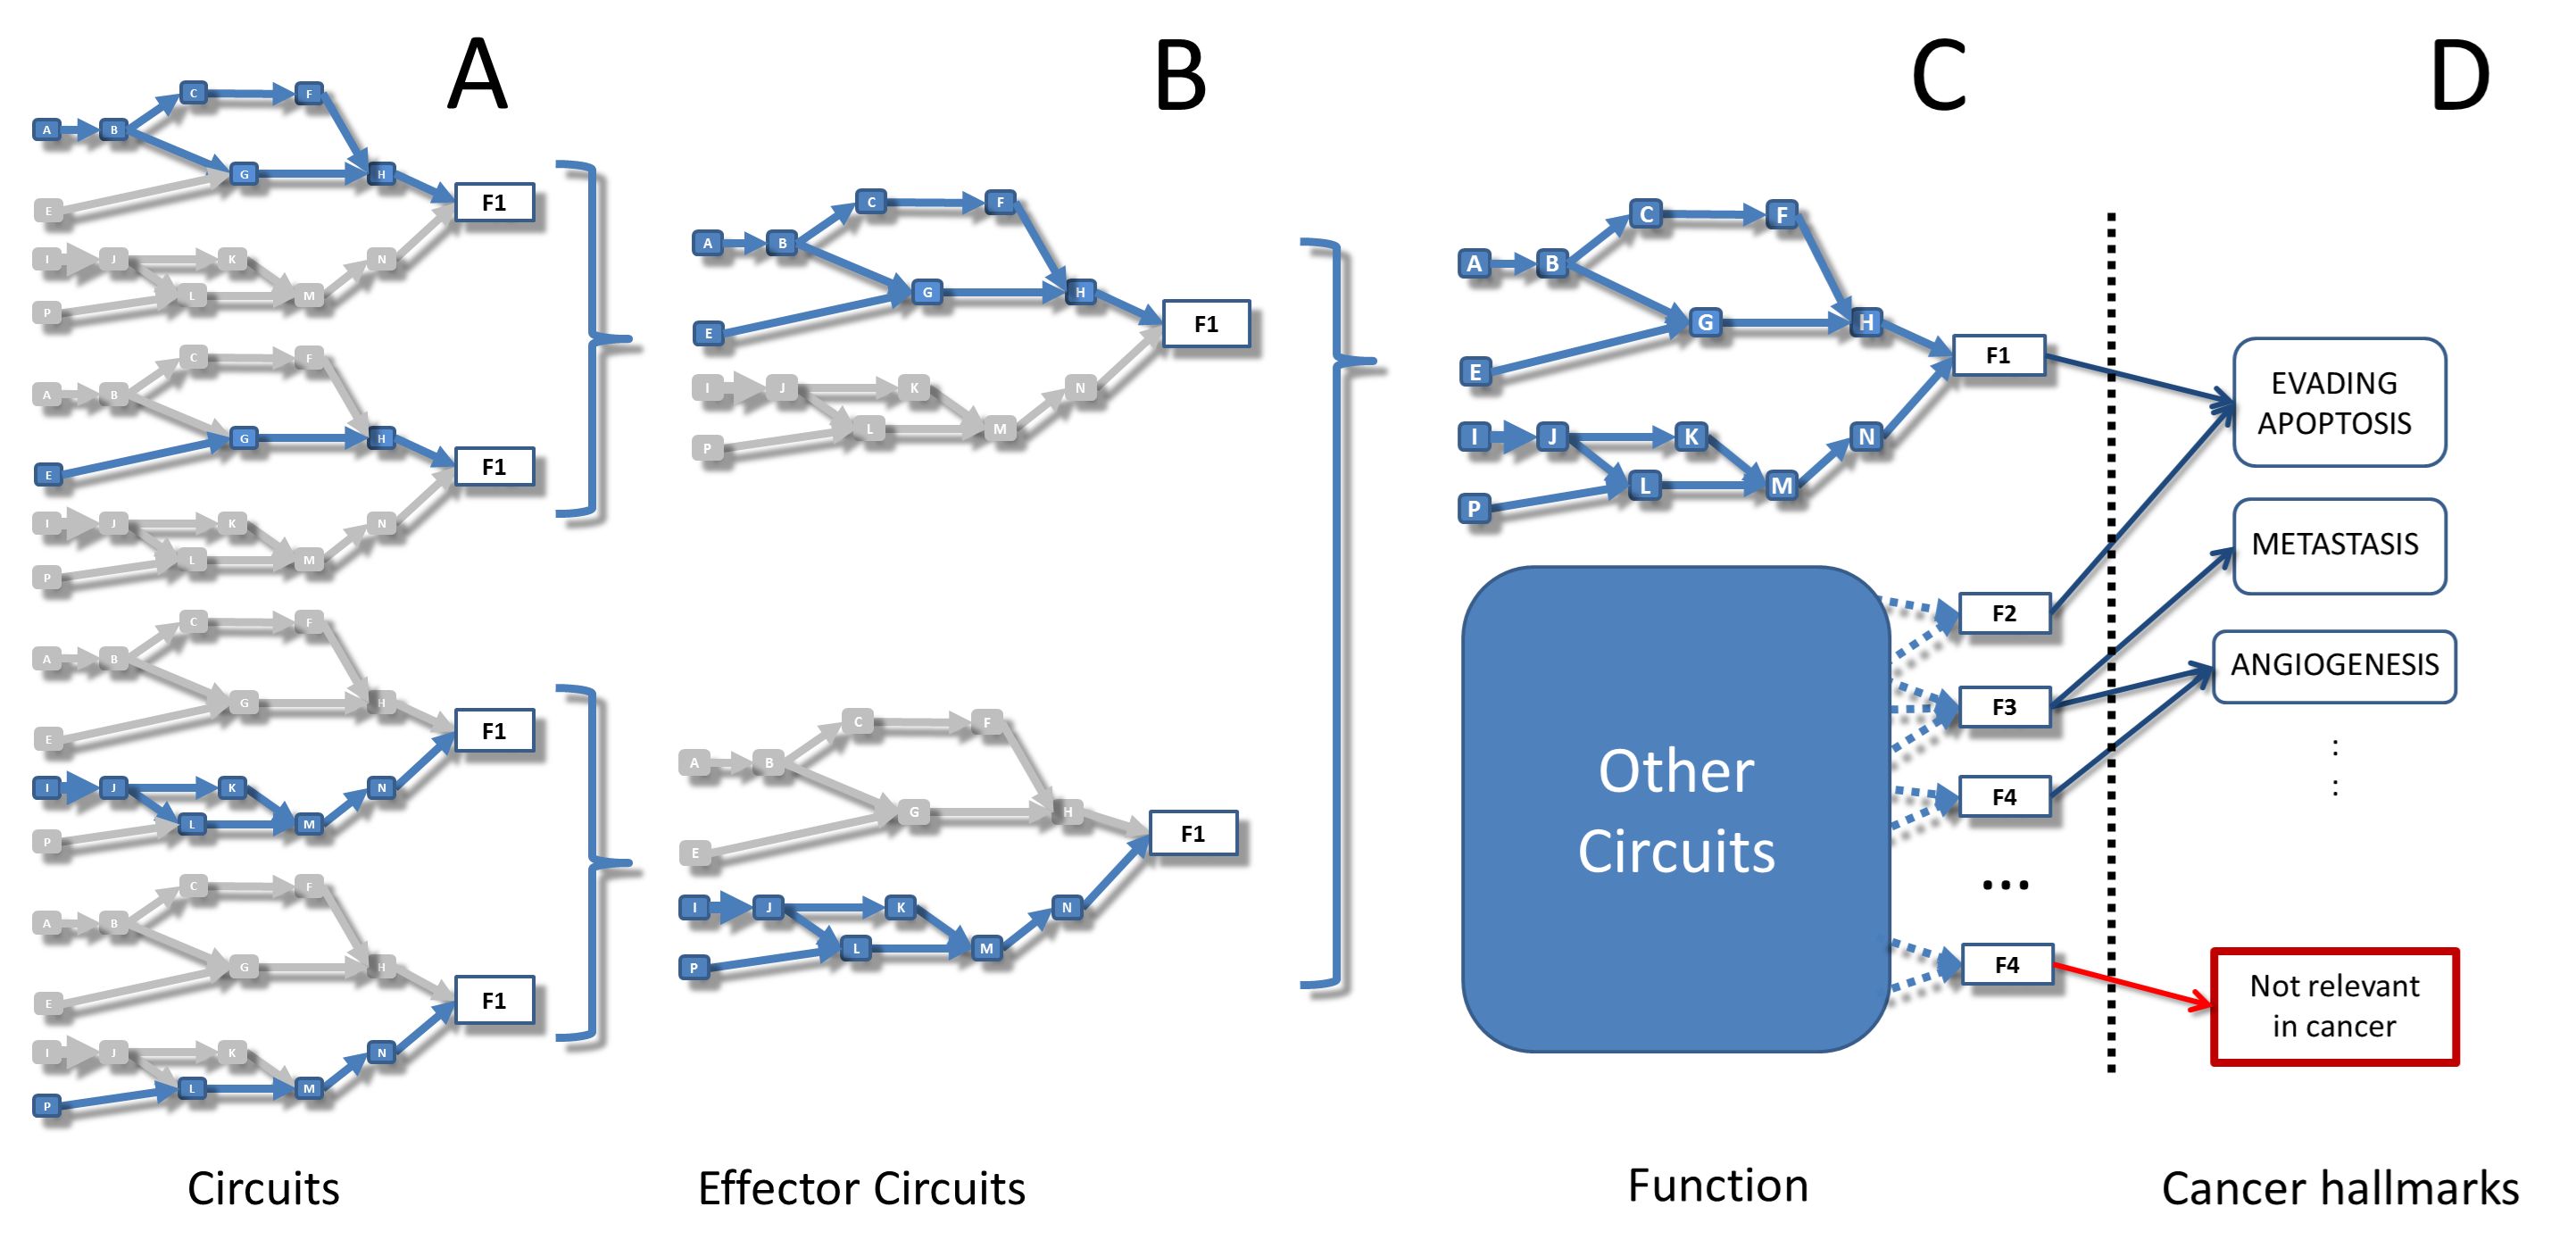
\includegraphics[width=\textwidth]{ch-hipathia/figure/pathway}
\caption{The different levels of abstraction within pathways: A) Circuits that communicate one receptor to one effector; B) Effector circuits that communicate all the receptors that signal a specific effector; C) Function circuits that collect the signal from all the effectors that trigger a specific function (according to UniProt or GO keywords); D) Cancer hallmarks, a sub-selection of only those functions related to cancer hallmarks.}
\label{fig4:pathway}
\end{figure}

In a signaling circuit, the transmission of the signal depends on the integrity of the chain of nodes that connect the receptor to the effector and the capability of transmitting signals of each node involved intuitively depends on two folds: the abundance of the proteins corresponding to that node and its activity status due to the interaction with its parent nodes. First, we need to estimate a value for each node in the pathways in regard to the presence of proteins involved in the node. Following the convention of \cite{Bhardwaj2005Correlation, Efroni2007Identification, Montaner2009Gene, Sebastian-Leon2014Understanding}, the presence of the mRNA (the normalized RNA-seq counts rescaled between 0 and 1) is taken as a proxy for the presence of the proteins involved in each node. Notably, for different types of nodes defined in KEGG, the value of a plain node in the pathways is defined as the ninetieth percentile of the values of the proteins contained, and the value of a complex node is taken as the minimum value of the proteins contained (the limiting component of the complex). Then, the degree of integrity of the circuit is estimated by modeling the signal flow across it, transmitting node-by-node following the path while its intensity value gets propagated along the way taking into account the current node value and the intensity of the signals arriving to it. Specifically, we initialize an incoming signal of intensity value of $1$ received by the input (receptor) node of the circuit, and then for each node $n$ of the circuit, the signal value $s_n$ is updated by the following rule:
$$
s_n = v_n \cdot \left( 1 - \prod_{a \in A_n} (1-s_a) \right) \cdot \prod_{i \in I_n} (1-s_i) \,,
$$
where $A_n$ denotes the set of signals arriving to the current node $n$ from activation edges, $I_n$ denotes the set of signals arriving to the current node $n$ from inhibition edges, and $v_n$ is the (normalized) value of the current node $n$. In case of loops present in the circuit, a node may be visited multiple times, until the difference in the updates of the signal value at that node is below certain threshold, before the signal exits the loop and continues to propagate down the cascade. Finally, the activity value for the circuit is defined by the signal intensity transmitted through the last (effector) protein of the circuit which quantifies the cell function ultimately activated by the circuit. See Figure \ref{fig4:hipathia} for an example of deducing the activity value of an artificial circuit by the \textit{hiPathia} method.

\begin{figure}[!htbp]
	\centering
	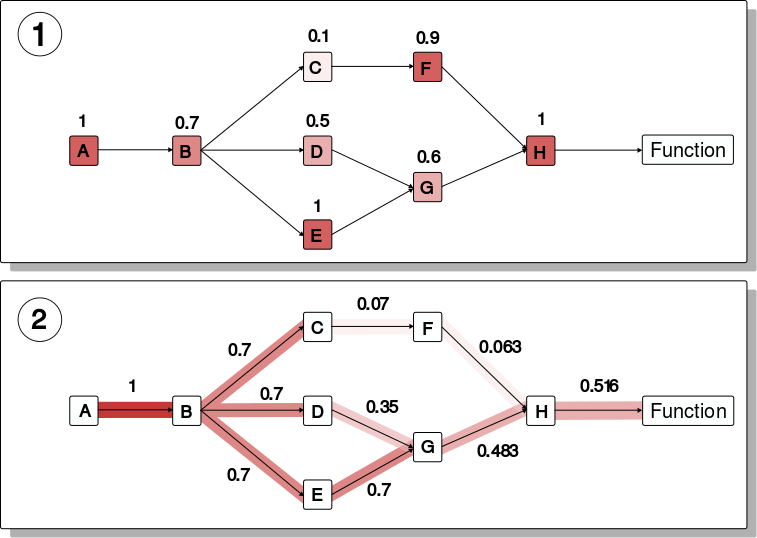
\includegraphics[width=0.6\textwidth]{ch-hipathia/figure/pretty_algorithm2}
	\caption{An example of computing the activity value of an artificial circuit by the \textit{hiPathia} method. In Step 1, node values are derived from the normalized mRNA measurements. In Step 2, signal is propagated along the path while its intensity value gets updated according to the rule of the \textit{hiPathia} method. Finally, The signal value attained after the last protein is visited accounts for the signaling activity of the circuit.}
	\label{fig4:hipathia}
\end{figure}

Besides, the \textit{hiPathia} method straightforwardly allows to explore pathway-level analysis at different levels of abstraction by applying to different notions of signaling circuits. As the output nodes at the end of circuits are the ultimate responsible to carry out specific cellular actions, an \textit{effector circuit} is defined from a functional viewpoint as a higher-level signaling entity that compose all circuits ending at the same output node (Figure \ref{fig4:pathway}, B). When applied to an effector circuit, the \textit{hiPathia} method returns the joint intensity of the signal arriving to the corresponding effector node. Furthermore, the known functions triggered in cell by each effector protein can be derived from their functional annotations. Here we use UniProt \cite{Consortium2015UniProt} and Gene Ontology (GO) \cite{Consortium2015Gene} annotations. Finally, inferred signaling activity values of those effector circuits ending at proteins with the same annotated functions are averaged to quantify the activity of the function realized in cell. This way we obtain estimated activity values directly connected to a list of cellular functions (Figure \ref{fig4:pathway}, C). Figure \ref{fig4:pathway} depicts the different levels of abstraction from circuits, to effector circuits and finally functions. Eventually for the sake of interpretation, a subset of curated functions can be used for a specific scenario in which the relevant functions are known to interpret the cancer biology, for which we use cancer hallmarks \cite{Hanahan2011Hallmarks} (Figure \ref{fig4:pathway}, D).

\subsection{Cancer Prognosis with Inferred Signaling Pathway Activity}
\label{sec4:prognosis}

In this study, we are interested in comparing the prognostic power of pathway-level mechanistic features and gene-based features, both separately and in combination, in order to distinguish good vs poor prognosis. Using the \textit{hiPathia} method, we recoded the list of gene expression values of each tumor sample into the corresponding lists of signaling activity values for the three levels of abstraction: circuits, effector circuits and functions, as described in UniProt and GO annotations. Therefore for each tumor sample, we end up with a profile of gene expression, a profile of circuit signaling activity, a profile of effector circuit signaling activity, a profile of UniProt-based cellular function activity and a profile of GO-based cellular function activity. These profiles are sample-specific, or so-called \textit{personalized}, profiles that can be straightforwardly used as prognostic features for cancer prognosis following any off-the-shelf classification algorithm. Note that pathway-level profiles are derived with no regard to any information provided by the genes whose products do not participate in cell signaling, and the prognostic power of pathway-level profiles may thus be limited by the coverage of genes in known biological pathways. In order to understand the relative contribution to the pathway-level profiles and gene-level profiles to the accurate separation between good vs poor prognosis, we devised 4 artificial profiles: path-gene expression profile containing only genes that are involved in the KEGG signaling pathways, other-gene expression profile containing only genes that are absent from the KEGG pathways, a combined profile consisting of signaling activity of effector circuits and expression of other-genes, and a combined profile consisting of signaling activity of circuits and expression of other-genes. Thus we obtained a total of 9 types of profiles (detailed in Table \ref{tab4:profile}).

\begin{table}[!htbp]
	\centering
	\caption{Summary of 9 different types of profiles used as predictive features for breast cancer prognosis.}
	\renewcommand{\arraystretch}{1.3}
	\begin{tabular}{|p{2.6cm}|p{3.5cm}|>{\raggedleft\arraybackslash}p{1.6cm}|m{4.8cm}|}
		\hline
		\textbf{Alias} & \textbf{Profile type} & \textbf{No. of features} & \textbf{Analysis level} \\\hline
		\textit{fun.vals} & UniProt-based functions & 81 & \multirow{2}{*}{\parbox{4.5cm}{\raggedright Pathway-level cellular function values}} \\
		\textit{go.vals} & GO-based functions & 370 &  \\
		\hline
		\textit{eff.vals} & Effector circuits & 1,038 & \multirow{2}{*}{\parbox{4.5cm}{\raggedright Pathway-level signaling activity values}} \\
		\textit{path.vals} & Circuits & 6,101 &  \\
		\hline
		\textit{path.genes.vals} & Path-genes & 2,212 & \multirow{3}{*}{\parbox{4.5cm}{\raggedright Gene-level expression values}} \\
		\textit{other.genes.vals} & Other-genes & 16,496 &  \\
		\textit{genes.vals} & All genes & 18,708 &  \\
		\hline
		\textit{eff.and.other.-genes.vals} & Effector circuits and other-genes & 17,534 & \multirow{2}{*}{\parbox{4.8cm}{\raggedright Combination of pathway-level signaling activity values and gene-level expression values}} \\
		\textit{path.and.other.-genes.vals} & Circuits and other-genes & 22,597 &  \\
		\hline
	\end{tabular}
	\label{tab4:profile}
\end{table}

From the viewpoint of machine learning, this study is formulated as a typical binary classification problem where we determine a positive or negative pseudo label for each sample. Based on the data available in this study (Table \ref{tab4:survival}), we perform a 5-fold cross-validation repeated 10 times on the dataset and report the mean performance over the $5 \times 10 = 50$ splits to assess the prognostic power for each type of profile. The performance is evaluated by the Area Under the ROC Curve (AUROC) criteria \cite{Sing2005ROCR}. Note that usually a classifier returns a continuous prediction between 0 and 1 for each sample denoting the probability of that sample being in the positive class rather than in the negative class, and then assigns either label to the sample according to some cutoff value thresholding the prediction. AUROC is a cutoff-free score that measures the probability that the classifier will score a randomly drawn positive sample higher than a randomly drawn negative sample.

In this study, we considered a total of 12 classification algorithms as candidate classifiers, most of which are state-of-the-art (Table \ref{tab4:classifier}). When we assess the prognosis performance for a specific type of profile on a specific (external) cross-validation split of the data, we perform an internal 5-fold cross-validation on the training set to determine which classifier returns the highest cross-validated performance and the best classifier is then used on the test set to obtain the performance score. The rationale behind the nested cross-validation is that, although any classification algorithm from the machine learning literature can be used to discriminate good vs poor prognosis with any profile type considered as predictive features, in practice, however, we do not have a definitive concept of which classifier suits the best universally for all types of profiles. In other words, it will be a confusing factor if we predetermine just one classifier throughout the study. In fact, the underlying hypotheses of different classifiers vary, for instance linear or non-linear relationships can be assumed between features and labels, and some classifiers can be particularly sensitive to the presence of a large number of noisy features. As a consequence, the procedure of choosing the best suited algorithm for different types of profiles by a nested cross-validation guarantees that the prediction performance is evaluated in an impartial fashion.

\begin{table}[!htbp]
	\centering
	\caption{The 12 candidate classifiers used to discriminate prognosis classes for breast tumor samples.}
	\renewcommand{\arraystretch}{1.3}
	\begin{tabularx}{\textwidth}{|l|X|X|}
		\hline
		\textbf{Alias} & \textbf{Classifier} & \textbf{Reference} \\\hline
		\textit{LDA} & Linear discriminant analysis & \cite{Venables2002Modern, Ripley2007Pattern} \\\hline
		\textit{LogitLasso} & L1-regularized logistic regression & \cite{Friedman2010Regularization} \\\hline
		\textit{LinearSVM} & Support Vector Machines with linear kernel & \cite{Chang2011LIBSVM} \\\hline
		\textit{RadialSVM} & Support Vector Machines with Gaussian RBF kernel & \cite{Chang2011LIBSVM} \\\hline
		\textit{KendallSVM} & Support Vector Machines with Kendall kernel & \cite{Zeileis2004kernlab, Jiao2015Kendall} \\\hline
		\textit{KNN} & $k$-nearest neighbor classifier & \cite{Venables2002Modern, Ripley2007Pattern} \\\hline
		\textit{NB} & Naive Bayes classifier & \cite{Ripley2007Pattern} \\\hline
		\textit{GBM} & Gradient Boosting Machines & \cite{Friedman2001Greedy} \\\hline
		\textit{RF} & Random Forests & \cite{Liaw2002Classification, Breiman2001Random} \\\hline
		\textit{SparseSVM} & L1-regularized L2-loss Support Vector Machines & \cite{Fan2008LIBLINEAR} \\\hline
		\textit{PAM} & Nearest shrunken centroid classifier & \cite{Tibshirani2002Diagnosis} \\\hline
		\textit{Constant} & Majority voting classifier & Outputs constant label of the dominant class (negative-control) \\\hline
	\end{tabularx}
	\label{tab4:classifier}
\end{table}



\section{Results}
\label{sec4:results}

\subsection{Signaling Pathway Activity Leads to Improved Prognosis for Breast Tumor Samples}
\label{sec4:performance}

The performance of using different types of profiles (Table \ref{tab4:profile}) as predictive features to classify survival outcome for breast cancer patients is shown in Figure \ref{fig4:score} while mean scores with standard deviation are reported in Table \ref{tab4:score}. Under the criterion of AUROC to evaluate the classification performance, we observe that the activity values of signaling circuits, denoted by  \textit{path.vals}, yield the best performance overall. In particular, they outperform the profiles based solely on gene expression values, denoted by \textit{path.genes.vals}, \textit{other.genes.vals} and \textit{genes.vals}. In other words, we are able to integrate the expression values of path-genes with the prior knowledge of cell signaling to obtain pathway-level features that achieve improved prognosis. Interestingly, these pathway-level features relate to biological processes and cellular functions \textit{per se}. Although the pathway-level features are derived from the expression of path-genes and thus agnostic to the expression of other-genes, the inclusion of other-genes to the signaling circuits, inducing the profiles denoted by \textit{eff.and.other.genes.vals} and \textit{path.and.other.genes.vals}, does not significantly improve the performance by performing a two-sided t-test comparing the difference between the cross-validation AUROC scores obtained by each pair of profiles further FDR-adjusted for multiple testing \cite{Benjamini1995Controlling} (Table \ref{tab4:test}).

\begin{figure}[!htbp]
	\centering
	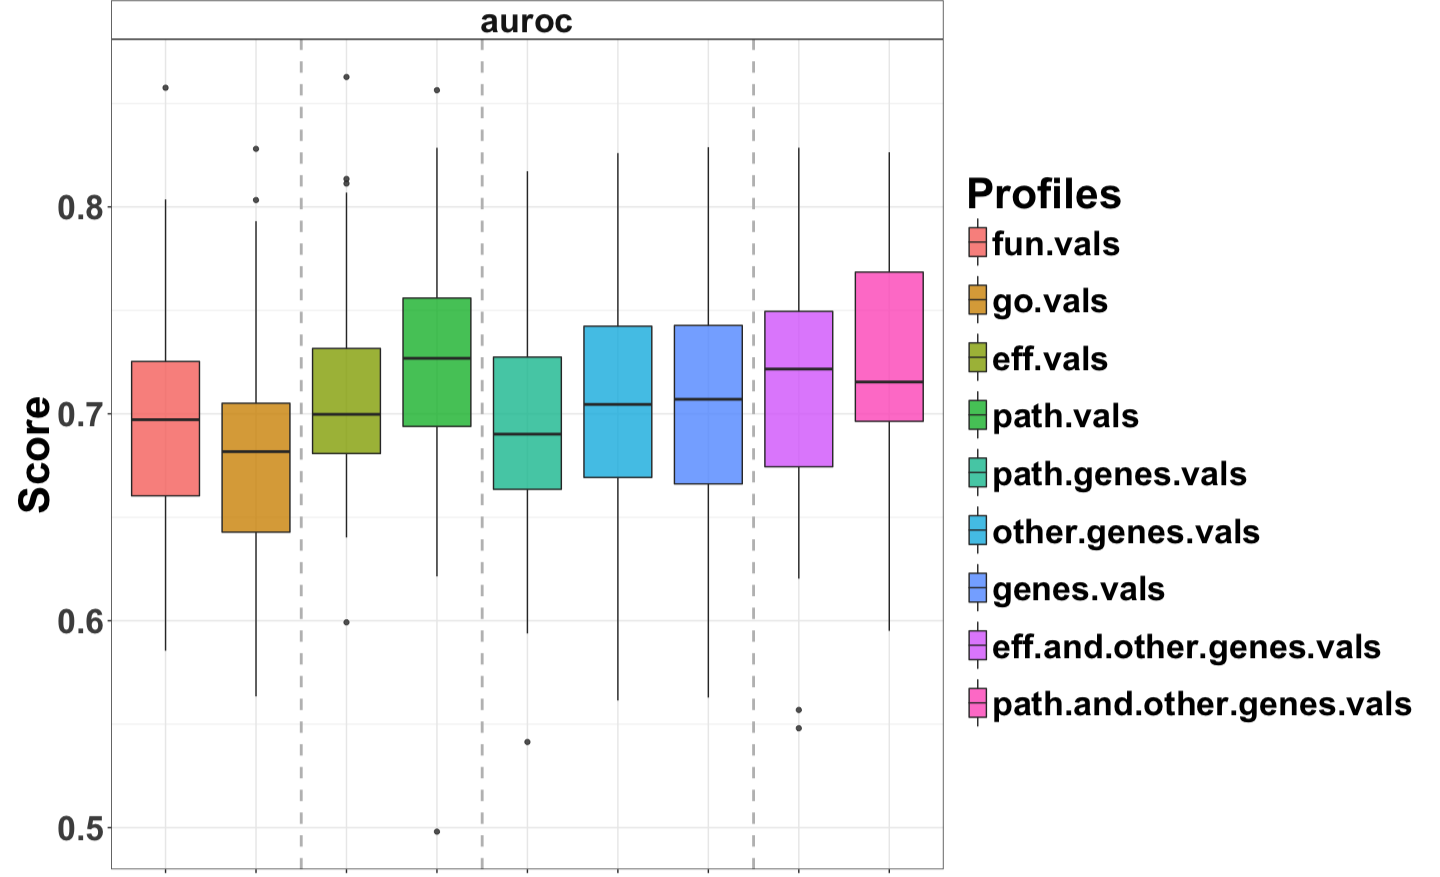
\includegraphics[width=0.8\textwidth]{ch-hipathia/results/score}
	\caption{The AUROC performance of using different types of profiles as predictive features to classify survival outcome for breast cancer patients. Boxplot represents the variance of the performance on 50 cross-validation splits. Dotted vertical lines separate profiles by the underlying analysis levels.}
	\label{fig4:score}
\end{figure}

\begin{table}[!htbp]
	\centering
	\caption{Mean AUROC scores with standard deviation (SD) and the top 2 most frequently selected classifiers by internal cross-validation for each type of prognostic profile in classifying breast cancer prognosis.}
	\begin{tabular}{|l|r|r|l|l|}
		\hline
		\textbf{Profile alias} & \textbf{Mean} & \textbf{SD} & \textbf{Classifier 1} & \textbf{Classifier 2} \\\hline
		\textit{fun.vals} & 0.6962 & 0.05438 & \textit{RadialSVM} & \textit{GBM} \\\hline
		\textit{go.vals} & 0.6807 & 0.06095 & \textit{RadialSVM} & \textit{LinearSVM} \\\hline
		\textit{eff.vals} & 0.7087 & 0.05099 & \textit{RadialSVM} & \textit{LinearSVM} \\\hline
		\textit{path.vals} & 0.7211 & 0.06316 & \textit{RadialSVM} & \textit{LinearSVM} \\\hline
		\textit{path.genes.vals} & 0.6938 & 0.05636 & \textit{RadialSVM} & \textit{LinearSVM} \\\hline
		\textit{other.genes.vals} & 0.7075 & 0.05254 & \textit{LinearSVM} & \textit{RadialSVM} \\\hline
		\textit{genes.vals} & 0.7075 & 0.05272 & \textit{LinearSVM} & \textit{RadialSVM} \\\hline
		\textit{eff.and.other.genes.vals} & 0.7127 & 0.05838 & \textit{LinearSVM} & \textit{RadialSVM} \\\hline
		\textit{path.and.other.genes.vals} & 0.7246 & 0.05359 & \textit{LinearSVM} & \textit{RadialSVM} \\\hline
	\end{tabular}
	\label{tab4:score}
\end{table}

\begin{sidewaystable}
	\centering
	\caption{FDR-adjusted p-values comparing the difference between the corresponding AUROC scores of profiles in columns and profiles in rows over 50 cross-validation splits. See Table \ref{tab4:score} for the mean scores of each profile individually. Significant p-values are boldfaced and marked with asterisks.}
	\renewcommand{\arraystretch}{1.3}
	\newcolumntype{R}{>{\raggedleft\arraybackslash}X}%
	\newcolumntype{L}{>{\raggedright\arraybackslash}X}%
	\begin{tabularx}{\textwidth}{|L|*{9}{R|}}
		\hline
		& \textit{go.vals} & \textit{eff.vals} & \textit{path.vals} & \textit{path.genes.-vals} & \textit{other.genes.-vals} & \textit{genes.vals} & \textit{eff.and.-other.-genes.vals} & \textit{path.and.-other.-genes.vals} \\\hline
		\textit{fun.vals} & 0.1467 & 0.1306 & \textbf{0.0119*} & 0.8267 & 0.1908 & 0.1908 & 0.0815 & \textbf{0.0020**} \\\hline
		\textit{go.vals} &  & \textbf{0.0024**} & \textbf{0.0004***} & 0.1557 & \textbf{0.0120*} & \textbf{0.0119*} & \textbf{0.0046**} & \textbf{$<$0.0001***} \\\hline
		\textit{eff.vals} &  &  & 0.0815 & \textbf{0.0255*} & 0.8743 & 0.8743 & 0.6422 & \textbf{0.0235*} \\\hline
		\textit{path.vals} &  &  &  & \textbf{0.0046**} & 0.1408 & 0.1394 & 0.3702 & 0.6422 \\\hline
		\textit{path.genes.-vals} &  &  &  &  & \textbf{0.0255*} & \textbf{0.0255*} & \textbf{0.0046**} & \textbf{0.0002***} \\\hline
		\textit{other.genes.-vals} &  &  &  &  &  & 0.9483 & 0.2167 & \textbf{0.0039**} \\\hline
		\textit{genes.vals} &  &  &  &  &  &  & 0.2000 & \textbf{0.0032**} \\\hline
		\textit{eff.and.-other.-genes.vals} &  &  &  &  &  &  &  & \textbf{0.0473*} \\\hline
	\end{tabularx}
	\label{tab4:test}
\end{sidewaystable}

When comparing the prognostic power between pathway-level and gene-level profiles, we have also derived cellular function activity profiles, denoted by \textit{fun.vals} and \textit{go.vals} (Table \ref{tab4:profile}), and observed that the performance of these profiles are slightly worse than other pathway-level profiles (Figure \ref{fig4:score}). This is probably due to the excessively simplistic procedure that basically averages the signaling activity values of effector circuits ending at proteins with the same annotated keywords according to UniProt or GO \cite{Hidalgo2017High}, annotations that can be incomplete and ambiguous to some extent.

Table \ref{tab4:score} summarizes the best-performing classifiers for each type of prognostic profile in the sense that they are most frequently selected by internal cross-validation. Notably, it evidences that Support Vector Machines with various kernels are recurrently selected as the competent classifier in breast cancer prognosis that suits well for both gene-level and pathway-level features.

\subsection{Signaling Circuits Selected as Features Relevant for Cancer Prognostic Account for Cancer Hallmarks}
\label{sec4:pathselect}

From the clinical standpoint of cancer prognosis, we are interested in identifying a small set of biomarkers that can guide decision making in cancer prognosis. As our analysis is made at the level of pathways, we would like to detect a few signaling circuits whose activity, and thus the underlying cell functionality, has a significant impact on discriminating the prognosis classes of cancer patients. We opted for the Random Forests classifier to perform this analysis, since it simultaneously predicts the survival outcome of tumor samples and scores the importance of each feature that is ultimately used in the prediction. We focus on the feature importance measure returned by fitting a Random Forest which accounts for the mean decrease in classification performance if we randomly permute the data of the corresponding feature.

Table \ref{tab4:path} lists the 5 top-scored circuits by fitting Random Forests with the profiles of circuit activities, denoted by \textit{path.vals}. The role played by each signaling circuit in cancer progression can be inferred from the underlying cellular functions (taken from GO annotations) triggered by the last (effector) protein on the circuit. Thus, the first circuit, belonging to the HIF-1 signaling pathway, starts with the TLR4 receptor, which is known to be related to progression of several cancers (breast, ovarian, prostate and head and neck) via lipopolysaccharide stimulation \cite{Yang2014Toll} and ends in the EDN1 effector, an hypoxia-inducible factor that mediates cancer progression \cite{Semenza2012Hypoxia}. Another relevant circuit belongs to the NF-kappa B signaling pathway and has the IL1B protein as receptor and the CXCL2 as effector. Polymorphisms in the receptor have been linked to several cancers in different populations \cite{El-Omar2000Interleukin, Lu2005Genetic} and it has been demonstrated the role of CXCL2 in tumor growth and angiogenesis \cite{Keane2004Depletion}. Similarly, polymorphisms in the LEP protein, the receptor of another circuit in the Adipocytokine signaling pathway, have been linked to cancer \cite{Cleveland2010Common}, and its effector, the tyrosine phosphatase Shp2 (PTPN11), contributes to the pathogenesis of many cancers and other human diseases \cite{Chan2008tyrosine}. The Cell cycle signaling pathway contains another relevant circuit whose receptor TTK transmits the signal until the cohesin complex. This four proteins complex is essential for chromosome segregation and DNA repair and mutations in its component genes have recently been identified in several types of tumors \cite{Losada2014Cohesin}. Finally, the last relevant circuit, belonging to the Tight junction pathway, contains the AKT3 serine/threonine kinase with a known role in tumorigenesis \cite{Testa2001AKT}, is signaled by the receptor ACTN4, a protein which has been related to cell invasion and metastasis \cite{Honda2015biological}. An expanded list of top-scored 50 circuits can be found in online supplementaries.

\begin{table}[!htbp]
	\centering
	\caption{Top 5 circuits with the highest feature importance measure by fitting Random Forests with \textit{path.vals} in classifying breast cancer prognosis, along their functions as annotated in Gene Ontology (GO).}
	\begin{tabularx}{\textwidth}{|l|X|X|X|X|}
		\hline
		\textbf{Rank} & \textbf{Pathway name} & \textbf{Receptor genes} & \textbf{Effector genes} & \textbf{Effector protein GO function} \\\hline
		1 & HIF-1 signaling pathway & TLR4 & EDN1 & Growth/survival factor in cancer \\\hline
		2 & NF-kappa B signaling pathway & IL1B & CXCL2 & Inflammatory response and angiogenesis \\\hline
		3 & Adipocytokine signaling pathway & LEP & PTPN11 & Protein phosphatase \\\hline
		4 & Cell cycle & TTK & Cohesin complex (SMC1B, SMC3, STAG1, RAD21) & Chromosome segregation and DNA repair \\\hline
		5 & Tight junction & ACTN4, MAGI3 & AKT3 & Cell invasion and metastasis \\\hline
	\end{tabularx}
	\label{tab4:path}
\end{table}

Table \ref{tab4:eff} lists the 5 top-scored effector circuits by fitting Random Forests with the profiles of effector circuit activities, denoted by \textit{eff.vals}. Although the cohesion complex effector is again selected, the effector circuit level analysis provided a slightly different perspective of relevant aspects of signaling in cancer patient survival. Thus, two effector circuits with effector proteins LEPR and PPAR$\alpha$, from the AMPK and the Adipocytokine signaling pathways, respectively, are activators of the fatty acid metabolism. Two more effector pathways ending in the Interleukin 6 (IL6), related to inflammatory processes and immune response in the Toll-like receptor pathway, seem more likely to be involved in blocking the cell differentiation through the Pathways in cancer (KEGG ID hsa05200). Actually, it has been described that IL6 blocks apoptosis in cells during the inflammatory process, keeping them alive in toxic environments, but the same process protects cells from apoptosis and chemotherapeutic drugs during neoplastic growth \cite{Hodge2005role}. An expanded list of top-scored 50 effector circuits can be found in the online supplementaries.

\begin{table}[!htbp]
	\centering
	\caption{Top 5 effector circuits with the highest feature importance measure by fitting Random Forests with \textit{eff.vals} in classifying breast cancer prognosis, along their functions as annotated in Gene Ontology (GO).}
	\begin{tabularx}{0.9\textwidth}{|l|X|X|X|}
		\hline
		\textbf{Rank} & \textbf{Pathway name} & \textbf{Effector genes} & \textbf{Effector protein GO function} \\\hline
		1 & AMPK signaling pathway & LEPR & Regulation of fatty acid metabolism \\\hline
		2 & Adipocytokine signaling pathway & PPAR$\alpha$ & Peroxisome proliferation and fatty acid metabolism \\\hline
		3 & Pathways in cancer & IL6 & Blockage of differentiation, Anti-apoptosis \\\hline
		4 & Cell cycle & Cohesin complex (SMC1B, SMC3, STAG1, RAD21) & Chromosome segregation and DNA repair \\\hline
		5 & Toll-like receptor signaling pathway & IL6 & Inflamation, Immune response, Anti-apoptosis \\\hline
	\end{tabularx}
	\label{tab4:eff}
\end{table}

\subsection{The Classification Algorithm Suggests Additional Prognostic Genes That Do Not Code for Signaling Proteins}
\label{sec4:othergene}

In order to find genes that could be relevant for patient survival that are not in the signal pathways, we have constructed a profile by combining signaling circuit activity profiles and gene expression profiles corresponding to other-genes absent from signaling pathways, denoted by \textit{path.and.other.genes.vals}. A feature selection procedure in breast cancer prognosis based on such a profile can select signaling circuits along with genes whose activity is unrelated to cell signaling but nonetheless related to patient survival. To this end, Random Forests was again used to score feature importance when fitted with the \textit{path.and.other.genes.vals} profile in the classification of breast cancer survival outcome.

Table \ref{tab4:othergene} lists the 5 top-scored other-genes that are part of the \textit{path.and.other.genes.vals} composed profile. These genes are of particular interest given that they might represent relevant cancer processes not included in cell signaling. Notably, the gene ABCB5 belongs to the ATP-binding cassette subfamily B which is well known to be involved in multiple drug resistance in cancer therapy \cite{Dean2001human}, probably due to its functionality of efflux transmembrane transporter. It has also been reported that ABCB5 could mediate cell-to-cell fusion and contribute to breast cancer chemoresistance in expressing breast tumors \cite{Frank2003Regulation, Frank2005ABCB5}. In addition, ABCB5, as a ``pro-survival'' gene, has been suggested to be a potential target against drug resistant breast cancer cells \cite{Yang2010p}. Besides, ABCB5 has been linked to melanoma \cite{Wilson2014ABCB5}. LMO4 encodes a LIM-domain protein that has been reported as an essential mediator of cell cycle progression in ErbB2/HER2/Neu-induced breast cancer which is characterized by poor survival due to high proliferation and metastasis rates \cite{Montanez-Wiscovich2009LMO4, Matthews2013LIM}. It has been reported that LMO4 interacts with the renowned tumor suppressor BRCA1 and inhibits BRCA1 activity \cite{Sum2002LIM, Sutherland2003Mutational}. OPA1 encodes a mitochondrial fusion protein which might be a target for mitochondrial apoptotic effectors \cite{Olichon2003Loss}, such as sorafenib \cite{Zhao2013OPA1}. The role in cancer survival played by two most important genes according to the results, VPS72 and CHADL, is not as clear from the literature. It is worth mentioning that a mutation in VPS72 in cervix cancer with a high FATHMM pathogenicity score \cite{Shihab2015integrative} is described in the COSMIC database (entry COSM458603). Regarding CHADL, it has been related to chondrocyte differentiation \cite{Tillgren2015novel} and extracellular matrix remodeling \cite{Barallobre-Barreiro2012Proteomics}. Therefore, both genes are potentially involved in cancer processes, which suggest that further investigation of the complete list of top-ranked other-genes could render new cancer drivers and potential therapeutic targets. An expanded list containing the top 50 most important features among the other-genes can be found in online supplementaries, in which many genes with cancer-related functions\footnote{Functions for those genes were taken from their UniProt annotations and, when absent, from GeneCards annotations \cite{Stelzer2016genecards}.} can be seen.

\begin{table}[!htbp]
	\centering
	\caption{Top 5 other-genes (genes unrelated to cell signaling) with the highest feature importance measure by fitting Random Forests with \textit{path.and.other.genes.vals} in classifying breast cancer prognosis, along their functions as annotated in Gene Ontology (GO).}
	\begin{tabularx}{\textwidth}{|l|l|l|X|X|}
		\hline
		\textbf{Rank} & \textbf{Gene ID} & \textbf{Gene symbol} & \textbf{Full name} & \textbf{GO function} \\\hline
		1 & 6944 & VPS72 & Vacuolar protein sorting 72 homolog & DNA binding \\\hline
		2 & 150356 & CHADL & Chondroadherin like & Collagen binding \\\hline
		3 & 340273 & ABCB5 & ATP binding cassette subfamily B member 5 & ATP binding, Efflux transmembrane transporter activity \\\hline
		4 & 8543 & LMO4 & LIM domain only 4 & Transcription factor activity, Sequence-specific DNA binding \\\hline
		5 & 4976 & OPA1 & OPA1, mitochondrial dynamin like GTPase & GTPase activity \\\hline
	\end{tabularx}
	\label{tab4:othergene}
\end{table}

\section{Discussion}
\label{sec4:discussion}

In this study we have proposed a novel scheme to classify survival outcome for breast cancer patients based on mechanistic features consisting of signaling pathway activity profiles. We applied a pathway activity analysis method \textit{hiPathia} \cite{Hidalgo2017High} to recode gene expression profiles into activity values of signaling circuits, and demonstrated that, making use of the state-of-the-art computational tools, signaling circuit activity yields better prediction in breast cancer prognosis than gene expression. An additional advantage is that the identified pathway-level biomarkers are mechanistic signatures whose contribution to cancer progression can be readily interpreted in terms of the underlying cellular functions and biological processes.

The three feature sets \textit{path.genes.vals}, \textit{eff.vals} and \textit{path.vals} are composed by the same set of genes, path-genes that are present in the pathways. However, pathway activity values recoded from these genes with the \textit{hiPathia} method, \textit{eff.vals} and \textit{path.vals}, clearly outperforms (see Table \ref{tab4:test}) the original path-genes, \textit{path.genes.vals}, in terms of prediction performance. Moreover, compared to the prediction performance with features based on all the genes, \textit{genes.vals}, that indeed carry more information than the subset of path-genes, features based on path-genes, \textit{path.genes.vals}, are significantly worse while features based on circuits of path-genes, \textit{eff.vals} and \textit{path.vals}, are competitive (see Table \ref{tab4:test}). It is worth noting that genes in the circuits assume only 12\% of the total number of genes. Therefore, it suggests that combining the genes into circuits provides a real added value for prediction purposes.

Although a significant improvement of the performance was not observed when the expression values of other-genes were concatenated to the activity values of signaling circuits, the analysis based on the combination of the two provides an interesting perspective regarding the interpretation of the biomarkers detected. In fact, the selected genes from the category of other-genes represent other aspects of the mechanism of the disease not explained by cell signaling. This approach allows expanding the scope of the analysis beyond the processes included in the pathways modeled.

Central to this study is the idea of promoting gene-level analysis to pathway-level analysis by obtaining personalized profiles of signaling circuit activity by applying the \textit{hiPathia} method. We deem that reliable models of pathway activity have the potential be used to derive robust multigenic biomarkers, in the spirit of renowned MammaPrint \cite{Veer2008Enabling}, which in addition account properly for the underlying disease mechanisms or mechanisms of drug action.

